\begin{enumerate}[label=\thesubsection.\arabic*, ref=\thesubsection.\theenumi]

\item A fair six-faced dice, with the faces labelled '1', '2', '3', '4', '5', and '6', is rolled thrice. What is the probability of rolling '6' exactly once?
\hfill (CS1~2025)
\begin{enumerate}
	\begin{multicols}{4}
    \item $\dfrac{75}{216}$
    \item $\dfrac{1}{6}$
    \item $\dfrac{1}{18}$
    \item $\dfrac{25}{216}$
	\end{multicols}
\end{enumerate}

\item A shop has 4 distinct flavors of ice-cream. One can purchase any number of scoops of any flavor. The order in which the scoops are purchased is inconsequential. If one wants to purchase 3 scoops of ice-cream, in how many ways can one make that purchase?
\hfill (CS1~2025)
\begin{enumerate}
	\begin{multicols}{4}
    \item $4$
    \item $20$
    \item $24$
    \item $48$
	\end{multicols}
\end{enumerate}

\item $g(\cdot)$ is a function from $A$ to $B$, $f(\cdot)$ is a function from $B$ to $C$, and their composition defined as $f(g(\cdot))$ is a mapping from $A$ to $C$. If $f(\cdot)$ and $f(g(\cdot))$ are onto (surjective) functions, which ONE of the following is TRUE about the function $g(\cdot)$?
\hfill (CS1~2025)
\begin{enumerate}
    \item $g(\cdot)$ must be an onto (surjective) function.
    \item $g(\cdot)$ must be a one-to-one (injective) function.
    \item $g(\cdot)$ must be a bijective function, that is, both one-to-one and onto.
    \item $g(\cdot)$ is not required to be a one-to-one or onto function.
\end{enumerate}

\item Let $G$ be any undirected graph with positive edge weights, and $T$ be a minimum spanning tree of $G$. For any two vertices, $u$ and $v$, let $d_1(u,v)$ and $d_2(u,v)$ be the shortest distances between $u$ and $v$ in $G$ and $T$, respectively. Which ONE of the options is CORRECT for all possible $G$, $T$, $u$ and $v$?
\hfill (CS1~2025)
\begin{enumerate}
	\begin{multicols}{2}
    \item $d_1(u,v) = d_2(u,v)$
    \item $d_1(u,v) \le d_2(u,v)$
    \item $d_1(u,v) \ge d_2(u,v)$
    \item $d_1(u,v) \ne d_2(u,v)$
	\end{multicols}
\end{enumerate}

\item Consider the following recurrence relation: $T(n) = 2T(n-1) + n 2^n$ for $n>0$, $T(0)=1$. Which ONE of the following options is CORRECT?
\hfill (CS1~2025)
\begin{enumerate}
	\begin{multicols}{2}
    \item $T(n) = \Theta(n^2 2^n)$
    \item $T(n) = \Theta(n 2^n)$
    \item $T(n) = \Theta((\log n)^2 2^n)$
    \item $T(n) = \Theta(4^n)$
	\end{multicols}
\end{enumerate}

\item Consider the given system of linear equations for variables $x$ and $y$, where $k$ is a real-valued constant:
\begin{align*}
x + ky &= 1 \\
kx + y &= -1
\end{align*}
Which of the following option(s) is/are CORRECT?
\hfill (CS1~2025)
\begin{enumerate}
    \item There is exactly one value of $k$ for which the above system of equations has no solution.
    \item There exist an infinite number of values of $k$ for which the system of equations has no solution.
    \item There exists exactly one value of $k$ for which the system of equations has exactly one solution.
    \item There exists exactly one value of $k$ for which the system of equations has an infinite number of solutions.
\end{enumerate}

\item Let $X$ be a 3-variable Boolean function that produces output as '1' when at least two of the input variables are '1'. Which of the following statement(s) is/are CORRECT, where $a, b, c, d, e$ are Boolean variables?
\hfill (CS1~2025)
\begin{enumerate}
    \item $X(a,b,X(c,d,e)) = X(X(a,b,c),d,e)$
    \item $X(a,b,X(a,b,c)) = X(a,b,c)$
    \item $X(a,b,X(a,c,d)) = (X(a,b,a) \text{ AND } X(c,d,c))$
    \item $X(a,b,c) = X(a, X(a,b,c), X(a,c,c))$
\end{enumerate}

\item The number -6 can be represented as 1010 in 4-bit 2's complement representation. Which of the following is/are CORRECT 2's complement representation(s) of -6?
\hfill (CS1~2025)
\begin{enumerate}
	\begin{multicols}{2}
    \item 1000 1010 in 8-bits
    \item 1111 1010 in 8-bits
    \item 1000 0000 0000 1010 in 16-bits
    \item 1111 1111 1111 1010 in 16-bits
	\end{multicols}
\end{enumerate}

\item Let $S$ be the set of all ternary strings defined over the alphabet $\{a, b, c\}$. Consider all strings in $S$ that contain at least one occurrence of two consecutive symbols, that is, "aa", "bb" or "cc". The number of such strings of length 5 that are possible is \underline{\hspace{1cm}}.
\hfill (CS1~2025)

\item Consider the given function $f(x)$:
\begin{align*}
f(x) = \begin{cases} ax + b, & \text{for } x < 1 \\ x^3 + x^2 + 1, & \text{for } x \ge 1 \end{cases}
\end{align*}
If the function is differentiable everywhere, the value of $b$ must be \underline{\hspace{1cm}}.
\hfill (CS1~2025)

\item A box contains 5 coins: 4 regular coins and 1 fake coin. When a regular coin is tossed, the probability $P(\text{head})=0.5$ and for a fake coin, $P(\text{head})=1$. You pick a coin at random and toss it twice, and get two heads. The probability that the coin you have chosen is the fake coin is \underline{\hspace{1cm}}.
\hfill (CS1~2025)

\item The pseudocode of a function \texttt{fun()} is given below:
\begin{lstlisting}[language=C]
fun (int A[0,...,n-1]) {
    for i = 0 to n-2
        for j = 0 to n-i-2
            if (A[j] > A[j+1])
                then swap A[j] and A[j+1]
}
\end{lstlisting}
Let $A[0,\dots,29]$ be an array storing 30 distinct integers in descending order. The number of swap operations that will be performed, if the function \texttt{fun()} is called with $A[0,\dots,29]$ as argument, is \underline{\hspace{1cm}}.
\hfill (CS1~2025)

\item Consider the following C program:
\begin{lstlisting}[language=C]
#include <stdio.h>

void foo (int *p, int x) {
    *p = x;
}

int main() {
    int *z;
    int a = 20, b = 25;
    z = &a;
    foo (z, b);
    printf ("%d", a);
    return 0;
}
\end{lstlisting}
The output of the given C program is \underline{\hspace{1cm}}.
\hfill (CS1~2025)

\item Let $A$ be a $2\times2$ matrix as given:
\begin{align*}
A = \begin{bmatrix} 1 & 1 \\ 1 & -1 \end{bmatrix}
\end{align*}
What are the eigenvalues of the matrix $A^{13}$?
\hfill (CS1~2025)
\begin{enumerate}
	\begin{multicols}{2}
    \item $1, -1$
    \item $2\sqrt{2}, -2\sqrt{2}$
    \item $4\sqrt{2}, -4\sqrt{2}$
    \item $64\sqrt{2}, -64\sqrt{2}$
	\end{multicols}
\end{enumerate}

\item Consider the following four variable Boolean function in sum-of-product form:
\begin{align*}
F(b_3,b_2,b_1,b_0) = \Sigma(0,2,4,8,10,11,12)
\end{align*}
where the value of the function is computed by considering $b_3 b_2 b_1 b_0$ as a 4-bit binary number, where $b_3$ denotes the most significant bit and $b_0$ denotes the least significant bit. Note that there are no don't care terms. Which ONE of the following options is the CORRECT minimized Boolean expression for $F$?
\hfill (CS1~2025)
\begin{enumerate}
	\begin{multicols}{2}
    \item $\overline{b}_1\overline{b}_0 + \overline{b}_2\overline{b}_0 + b_1\overline{b}_2 b_3$
    \item $\overline{b}_1\overline{b}_0 + \overline{b}_2\overline{b}_0$
    \item $\overline{b}_2\overline{b}_0 + b_1 b_2 b_3$
    \item $\overline{b}_0\overline{b}_2 + \overline{b}_3$
	\end{multicols}
\end{enumerate}

\item Let $G(V,E)$ be an undirected and unweighted graph with 100 vertices. Let $d(u,v)$ denote the number of edges in a shortest path between vertices $u$ and $v$ in $V$. Let the maximum value of $d(u,v)$, $u,v\in V$ such that $u\ne v$ be 30. Let $T$ be any breadth-first-search tree of $G$. Which ONE of the given options is CORRECT for every such graph $G$?
\hfill (CS1~2025)
\begin{enumerate}
	\begin{multicols}{2}
    \item The height of $T$ is exactly 15.
    \item The height of $T$ is exactly 30.
    \item The height of $T$ is at least 15.
    \item The height of $T$ is at least 30.
	\end{multicols}
\end{enumerate}

\item $A=\{0,1,2,3,\dots\}$ is the set of non-negative integers. Let $F$ be the set of functions from $A$ to itself. For any two functions, $f_1, f_2 \in F$ we define
\begin{align*}
(f_1 \odot f_2)(n) = f_1(n) + f_2(n)
\end{align*}
for every number $n$ in $A$. Which of the following is/are CORRECT about the mathematical structure $(F, \odot)$?
\hfill (CS1~2025)
\begin{enumerate}
	\begin{multicols}{2}
    \item $(F, \odot)$ is an Abelian group.
    \item $(F, \odot)$ is an Abelian monoid.
    \item $(F, \odot)$ is a non-Abelian group.
    \item $(F, \odot)$ is a non-Abelian monoid.
	\end{multicols}
\end{enumerate}

\item Refer to the given 3-address code sequence. This code sequence is split into basic blocks. The number of basic blocks is \underline{\hspace{1cm}}.
\hfill (CS1~2025)
\begin{lstlisting}[language=C]
1001: i = 1
1002: j = 1
1003: t1 = 10 * i
1004: t2 = t1 + j
1005: t3 = 8 * t2
1006: t4 = t3 - 88
1007: a[t4] = 0.0
1008: j = j + 1
1009: if j <= 10 goto 1003
1010: i = i + 1
1011: if i <= 10 goto 1002
1012: i = 1
1013: t5 = i - 1
1014: t6 = 88 * t5
1015: a[t6] = 1.0
1016: i = i + 1
1017: if i <= 10 goto 1013
\end{lstlisting}

\item Consider the following database tables of a sports league:
\begin{itemize}
    \item \texttt{player (pid, pname, age)}
    \item \texttt{coach (cid, cname)}
    \item \texttt{team (tid, tname, city, cid)}
    \item \texttt{members (pid, tid)}
\end{itemize}
An instance of the table and an SQL query are given below.

\vspace{0.2cm}
\begin{minipage}{0.48\textwidth}
\textbf{player} \\
\begin{tabular}{|c|c|c|}
\hline
pid & pname & age \\ \hline
1 & Jasprit & 31 \\
2 & Atharva & 24 \\
3 & Ishan & 26 \\
4 & Axar & 30 \\ \hline
\end{tabular}
\end{minipage}
\begin{minipage}{0.48\textwidth}
\textbf{coach} \\
\begin{tabular}{|c|c|}
\hline
cid & cname \\ \hline
101 & Ricky \\
102 & Mark \\
103 & Trevor \\ \hline
\end{tabular}
\end{minipage}

\vspace{0.3cm}
\begin{minipage}{0.55\textwidth}
\textbf{team} \\
\begin{tabular}{|c|c|c|c|}
\hline
tid & tname & city & cid \\ \hline
10 & MI & Mumbai & 102 \\
20 & DC & Delhi & 101 \\
30 & PK & Mohali & 103 \\ \hline
\end{tabular}
\end{minipage}
\begin{minipage}{0.4\textwidth}
\textbf{members} \\
\begin{tabular}{|c|c|}
\hline
pid & tid \\ \hline
1 & 10 \\
2 & 30 \\
3 & 10 \\
4 & 20 \\ \hline
\end{tabular}
\end{minipage}

\vspace{0.3cm}
\begin{lstlisting}[language=SQL]
SELECT MIN (P.age)
FROM player P
WHERE P.pid IN (
    SELECT M.pid
    FROM team T, coach C, members M
    WHERE C.cname = 'Mark'
      AND T.cid = C.cid
      AND M.tid = T.tid
)
\end{lstlisting}
The value returned by the given SQL query is \underline{\hspace{1cm}}.
\hfill (CS1~2025)

\item Suppose a 5-bit message is transmitted from a source to a destination through a noisy channel. The probability that a bit of the message gets flipped during transmission is 0.01. Flipping of each bit is independent of one another. The probability that the message is delivered error-free to the destination is \underline{\hspace{1cm}}.
\hfill (CS1~2025)

\item Consider a probability distribution given by the density function $P(x)$:
\begin{align*}
P(x) = \begin{cases} C x^2, & \text{for } 1 \le x \le 4 \\ 0, & \text{for } x < 1 \text{ or } x > 4 \end{cases}
\end{align*}
The probability that $x$ lies between 2 and 3, i.e., $P(2 \le x \le 3)$ is \underline{\hspace{1cm}}.
\hfill (CS1~2025)

\item Consider a finite state machine (FSM) with one input $X$ and one output $f$, represented by the given state transition table. The minimum number of states required to realize this FSM is \underline{\hspace{1cm}}.
\hfill (CS1~2025)

\begin{center}
\begin{tabular}{|c|c|c|c|c|}
\hline
\multirow{2}{*}{\textbf{Present state}} & \multicolumn{2}{c|}{\textbf{Next state}} & \multicolumn{2}{c|}{\textbf{Output f}} \\ \cline{2-5}
 & $X=0$ & $X=1$ & $X=0$ & $X=1$ \\ \hline
A & F & B & 0 & 0 \\
B & D & C & 0 & 0 \\
C & F & E & 0 & 0 \\
D & G & A & 1 & 0 \\
E & D & C & 0 & 0 \\
F & F & B & 1 & 1 \\
G & G & H & 0 & 1 \\
H & G & A & 1 & 0 \\ \hline
\end{tabular}
\end{center}

\item Consider the given sequential circuit designed using D-Flip-flops. The circuit is initialized with some value (initial state). The number of distinct states the circuit will go through before returning back to the initial state is \underline{\hspace{1cm}}.
\hfill (CS1~2025)

\begin{center}
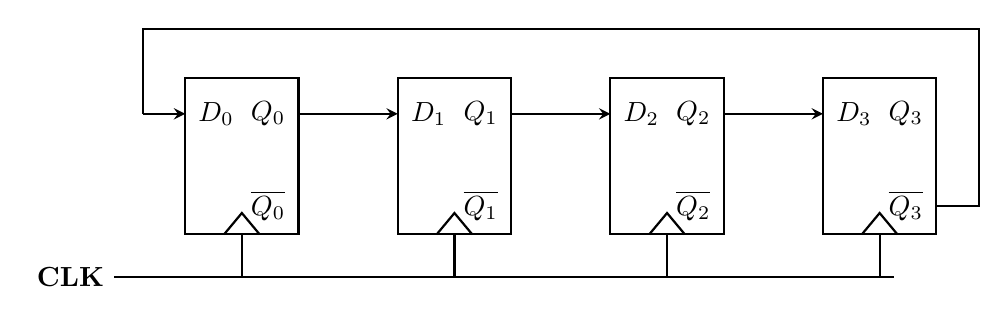
\begin{tikzpicture}[scale=0.9, >=stealth]
    \foreach \x/\i in {0/0, 3/1, 6/2, 9/3} {
        \draw[thick] (\x, 0) rectangle (\x+1.6, 2.2);
        \node[anchor=west] at (\x+0.05, 1.7) {$D_\i$};
        \node[anchor=east] at (\x+1.55, 1.7) {$Q_\i$};
        \node[anchor=east] at (\x+1.55, 0.4) {$\overline{Q_\i}$};
        \draw[thick] (\x+0.55, 0) -- (\x+0.8, 0.3) -- (\x+1.05, 0);
    }
    \draw[->, thick] (1.6, 1.7) -- (3.0, 1.7);
    \draw[->, thick] (4.6, 1.7) -- (6.0, 1.7);
    \draw[->, thick] (7.6, 1.7) -- (9.0, 1.7);
    \draw[thick] (10.6, 0.4) -- (11.2, 0.4) -- (11.2, 2.9) -- (-0.6, 2.9) -- (-0.6, 1.7);
    \draw[->, thick] (-0.6, 1.7) -- (0.0, 1.7);
    \draw[thick] (-1.0, -0.6) node[left] {\textbf{CLK}} -- (10.0, -0.6);
    \foreach \x in {0, 3, 6, 9} {
        \draw[thick] (\x+0.8, -0.6) -- (\x+0.8, 0.0);
    }
\end{tikzpicture}
\end{center}

\item Consider the following C program:
\begin{lstlisting}[language=C]
#include <stdio.h>

int foo (int S[], int size) {
    if (size == 0) return 0;
    if (size == 1) return 1;
    if (S[0] != S[1]) return 1 + foo(S + 1, size - 1);
    return foo(S + 1, size - 1);
}

int main() {
    int A[] = {0, 1, 2, 2, 2, 0, 0, 1, 1};
    printf ("%d", foo(A, 9));
    return 0;
}
\end{lstlisting}
The value printed by the given C program is \underline{\hspace{1cm}}.
\hfill (CS1~2025)

\item Let \texttt{LIST} be a datatype for an implementation of linked list defined as follows:
\begin{lstlisting}[language=C]
typedef struct list {
    int data;
    struct list *next;
} LIST;
\end{lstlisting}
Suppose a program has created two linked lists, L1 and L2, whose contents are given in the figure below (code for creating L1 and L2 is not provided here). L1 contains 9 nodes, and L2 contains 7 nodes.

\begin{center}
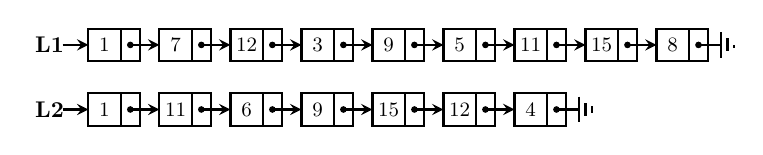
\begin{tikzpicture}[scale=0.82, transform shape, >=stealth]
    \node at (-0.6, 1) {\textbf{L1}};
    \draw[->, thick] (-0.4, 1) -- (0, 1);
    \foreach \val/\x in {1/0, 7/1.1, 12/2.2, 3/3.3, 9/4.4, 5/5.5, 11/6.6, 15/7.7, 8/8.8} {
        \draw[thick] (\x, 0.75) rectangle (\x+0.8, 1.25);
        \draw[thick] (\x+0.5, 0.75) -- (\x+0.5, 1.25);
        \node at (\x+0.25, 1) {\small \val};
        \filldraw (\x+0.65, 1) circle (1.2pt);
        \ifdim \x pt < 8.8pt
            \draw[->, thick] (\x+0.65, 1) -- (\x+1.1, 1);
        \fi
    }
    \draw[thick] (9.45, 1) -- (9.8, 1);
    \draw[thick] (9.8, 1.2) -- (9.8, 0.8);
    \draw[thick] (9.9, 1.1) -- (9.9, 0.9);
    \draw[thick] (10.0, 1.0) -- (10.0, 0.95);

    \node at (-0.6, 0) {\textbf{L2}};
    \draw[->, thick] (-0.4, 0) -- (0, 0);
    \foreach \val/\x in {1/0, 11/1.1, 6/2.2, 9/3.3, 15/4.4, 12/5.5, 4/6.6} {
        \draw[thick] (\x, -0.25) rectangle (\x+0.8, 0.25);
        \draw[thick] (\x+0.5, -0.25) -- (\x+0.5, 0.25);
        \node at (\x+0.25, 0) {\small \val};
        \filldraw (\x+0.65, 0) circle (1.2pt);
        \ifdim \x pt < 6.6pt
            \draw[->, thick] (\x+0.65, 0) -- (\x+1.1, 0);
        \fi
    }
    \draw[thick] (7.25, 0) -- (7.6, 0);
    \draw[thick] (7.6, 0.2) -- (7.6, -0.2);
    \draw[thick] (7.7, 0.1) -- (7.7, -0.1);
    \draw[thick] (7.8, 0.05) -- (7.8, -0.05);
\end{tikzpicture}
\end{center}

Consider the following C program segment that modifies the list L1. The number of nodes that will be there in L1 after the execution of the code segment is \underline{\hspace{1cm}}.
\hfill (CS1~2025)
\begin{lstlisting}[language=C]
int find (int query, LIST *list) {
    while (list != NULL) {
        if (list->data == query) return 1;
        list = list->next;
    }
    return 0;
}

int main () {
    ptr1 = L1; ptr2 = L2;
    while (ptr1->next != NULL) {
        query = ptr1->next->data;
        if (find (query, L2))
            ptr1->next = ptr1->next->next;
        else
            ptr1 = ptr1->next;
    }
    return 0;
}
\end{lstlisting}

\item Consider the following C program:
\begin{lstlisting}[language=C]
#include <stdio.h>

int gate (int n) {
    int d, t, newnum, turn;
    newnum = turn = 0; t = 1;
    while (n >= t) t *= 10;
    t /= 10;
    while (t > 0) {
        d = n / t;
        n = n % t;
        t /= 10;
        if (turn) newnum = 10 * newnum + d;
        turn = (turn + 1) % 2;
    }
    return newnum;
}

int main () {
    printf ("%d", gate (14362));
    return 0;
}
\end{lstlisting}
The value printed by the given C program is \underline{\hspace{1cm}}.
\hfill (CS1~2025)

\item The maximum value of $x$ such that the edge between the nodes B and C is included in every minimum spanning tree of the given graph is \underline{\hspace{1cm}}.
\hfill (CS1~2025)

\begin{center}
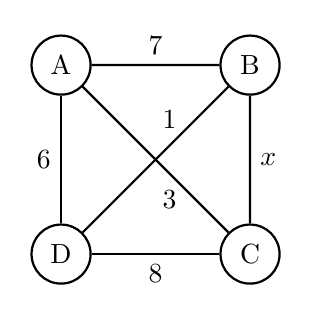
\begin{tikzpicture}[scale=1.2, >=stealth]
    \node[circle, draw, thick, minimum size=7.5mm, inner sep=0pt] (A) at (0, 2) {A};
    \node[circle, draw, thick, minimum size=7.5mm, inner sep=0pt] (B) at (2, 2) {B};
    \node[circle, draw, thick, minimum size=7.5mm, inner sep=0pt] (D) at (0, 0) {D};
    \node[circle, draw, thick, minimum size=7.5mm, inner sep=0pt] (C) at (2, 0) {C};

    \draw[thick] (A) -- node[above] {7} (B);
    \draw[thick] (A) -- node[left] {6} (D);
    \draw[thick] (D) -- node[below] {8} (C);
    \draw[thick] (B) -- node[right] {$x$} (C);

    \draw[thick] (D) -- node[pos=0.68, above left, fill=white, inner sep=1.5pt] {1} (B);
    \draw[thick] (A) -- node[pos=0.68, below left, fill=white, inner sep=1.5pt] {3} (C);
\end{tikzpicture}
\end{center}

\item In a double hashing scheme, $h_1(k) = k \bmod 11$ and $h_2(k) = 1 + (k \bmod 7)$ are the auxiliary hash functions. The size $m$ of the hash table is 11. The hash function for the $i$-th probe in the open address table is $[h_1(k) + i \cdot h_2(k)] \bmod m$. The following keys are inserted in the given order: 63, 50, 25, 79, 67, 24. The slot at which key 24 gets stored is \underline{\hspace{1cm}}.
\hfill (CS1~2025)

\end{enumerate}
